\documentclass[border=2pt]{standalone}
\usepackage{amsmath}
\usepackage{tikz}
\usetikzlibrary{arrows.meta}

\definecolor{orangeText}{HTML}{E3A063}
\definecolor{orangeDim}{HTML}{A87A4E}
\begin{document}
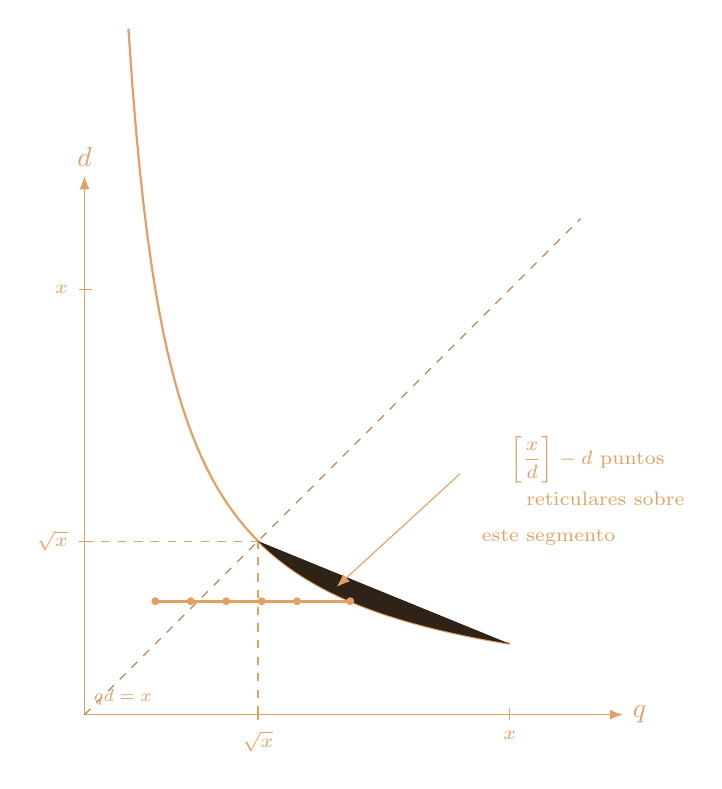
\begin{tikzpicture}[color=orangeText, >=Latex, scale=0.9]

    % axes
    \draw[->] (0,0) -- (7.6,0) node[right] {$q$};
    \draw[->] (0,0) -- (0,7.6) node[above] {$d$};

    % symmetry line q = d
    \draw[dashed, orangeDim] (0,0) -- (7,7);

    % hyperbola qd = x  (x = 6 here, drawn on domain giving nice shape)
    \draw[thick] plot[domain=0.62:6,samples=100] (\x,{6/\x}) node[pos=0,above right] {\scriptsize $qd=x$};

    % dashed reference lines at sqrt(x) and x
    \draw[dashed] (2.449,0) -- (2.449,2.449);
    \draw[dashed] (0,2.449) -- (2.449,2.449);
    \draw[dashed] (0,6) -- (0.1,6);
    \draw[dashed] (6,0) -- (6,0.1);

    % shaded region between the hyperbola and the symmetry line, for q in [sqrt x, x]
    \fill[orangeDim!28!black] plot[domain=2.449:6,samples=80] (\x,{6/\x}) -- (2.449,2.449) -- cycle;

    % horizontal segment illustrating lattice points at a fixed d
    \draw[very thick] (1,1.6) -- (3.75,1.6);
    \foreach \x in {1,1.5,2,2.5,3,3.75} {
        \fill (\x,1.6) circle (1.6pt);
    }
    \draw[->,shorten >=2pt] (5.3,3.4) -- (3.5,1.75);
    \node[align=left] at (7.1,3.6) {\scriptsize $\left[\dfrac{x}{d}\right]-d$ puntos};
    \node[align=left] at (7.35,3.05) {\scriptsize reticulares sobre};
    \node[align=left] at (6.55,2.5) {\scriptsize este segmento};

    % axis ticks
    \draw (2.449,-0.08) -- (2.449,0.08);
    \node[below] at (2.449,-0.1) {\scriptsize $\sqrt{x}$};
    \draw (6,-0.08) -- (6,0.08);
    \node[below] at (6,-0.1) {\scriptsize $x$};

    \draw (-0.08,2.449) -- (0.08,2.449);
    \node[left] at (-0.1,2.449) {\scriptsize $\sqrt{x}$};
    \draw (-0.08,6) -- (0.08,6);
    \node[left] at (-0.1,6) {\scriptsize $x$};

\end{tikzpicture}
\end{document}
